\section{Felder}
Materialgleichungen
\begin{align*}
    \Aboxed{\vec{J}  = \kappa\vec{E}} &
    \Aboxed{\vec{B}  = \mu\vec{H}}    &
    \Aboxed{\vec{D}  = \varepsilon\vec{E}}
\end{align*}

Feldunterscheidung
\begin{align*}
     & \vec{E}(x,y,z)                               & \widehat= & \quad\text{statisches Feld}  & \\
     & \vec{E}(x,y,z,t)                             & \widehat= & \quad\text{stationäres Feld} & \\
     & \vec{E}(x,y,z,t)\cdot cos(\omega t -\beta z) & \widehat= & \quad\text{Welle}            &
\end{align*}


\subsection{E-Felder an Grenzflächen}
\textbf{Dielektrische Grenzfläche}\\
\begin{tabularx}{0.45\textwidth}{>{\hsize=.3\hsize}X>{\hsize=.5\hsize}X}
    Querschichtung:   & $D_{1n} = D_{2n}$                                                                                                        \\
                      & ${\displaystyle\oiint} \vec{D} \cdot d \vec{a} = 0$                                                                      \\
    Längsschichtung:  & $E_{1t} = E_{2t}$                                                                                                        \\
                      & $ {\displaystyle\oint} \vec{E} \cdot d \vec{s} = 0$                                                                      \\
    Schrägschichtung: & $ \frac{\tan( \alpha_1)}{\tan( \alpha_2)} = \frac{E_{1t}/E_{1n}}{E_{2t}/E_{2n}} = \frac{ \varepsilon_1}{\varepsilon_2} $
\end{tabularx}

\textbf{Grenzfläche dielektrischer Leiter}\\
\begin{tabularx}{0.45\textwidth}{>{\hsize=.3\hsize}X>{\hsize=.5\hsize}X}
    Längsschichtung: & $E_{1t} = E_{2t}$                                   \\
                     & ${\displaystyle\oint} \vec{E} \cdot d \vec{s} = 0$  \\
    Querschichtung:  & $D_{1n} = \frac{Q}{A}$                              \\
                     & ${\displaystyle\oiint} \vec{D} \cdot d \vec{a} = Q$
\end{tabularx}

\textbf{Grenzfläche an magn. Feldern}\\
\begin{tabularx}{0.45\textwidth}{>{\hsize=.3\hsize}X>{\hsize=.5\hsize}X}
    Querschichtung:   & $B_{1n} = B_{2n}$                                                    \\
                      & ${\displaystyle\oiint} \vec{B} \cdot d \vec{a} = 0$                  \\
    Längsschichtung:  & $H_{1t} = H_{2t}$                                                    \\
                      & ${\displaystyle\oint} \vec{H} \cdot d \vec{s} = 0$                   \\
    Schrägschichtung: & $\frac{\tan( \alpha_1)}{\tan( \alpha_2)} = \frac{ \mu_1 }{ \mu_2 } $
\end{tabularx}

\subsection{Elektrostatik}
$\bullet$ wirbelfreies Feld $\rightarrow$ Elektrische Ladungen sind Quellen des
Feldes
\begin{align*}
    \opdiv \vec{D} & = \nabla \cdot \vec{D}  = \rho & \qquad \vec{D} & = \varepsilon \vec{E} \\
    \oprot \vec{E} & = \nabla \times \vec{E} = 0    & \qquad         & = \oprot \opgrad E
\end{align*}

Dipolmoment $\vec{p} = Q \cdot \vec{d}$
\begin{align*}
    \varphi & = \frac{Q}{4 \pi \varepsilon_0} \cdot \left(\frac{1}{r_1} - \frac{1}{r_2}\right) = \frac{Q}{4 \pi \varepsilon_0} \frac{\vec{p} \cdot \vec{r}}{r^3} \\
    \vec{E} & =- \opgrad \varphi = \frac{1}{4 \pi \varepsilon_0} \cdot \left( \frac{3( \vec{p} \cdot \vec{r}) \cdot \vec{r}}{r^5} - \frac{\vec{p}}{r^3}\right)
\end{align*}

\subsubsection{Potential Gleichung}
\[
    \opdiv \opgrad \varphi = - \dfrac{\rho}{\varepsilon}
\]

\textbf{$\qquad \Rightarrow$ Poisson-Gleichung} mit $\rho = 0$

$\rightarrow$ \textbf{Laplace-Gleichung}
\begin{align*}
    \Delta \varphi + \underbrace{ \dfrac{\opgrad \varepsilon \cdot \opgrad \varphi}{\varepsilon}}_{= 0\texttt{, wenn homogen}}
     & = - \dfrac{\rho (x, y, z)}{\varepsilon} \\
    \frac{d^2 \varphi}{d x^2} + \frac{d^2 \varphi}{d y^2} + \frac{d^2 \varphi}{d z^2}
     & = - \dfrac{\rho (x, y, z)}{\varepsilon}
\end{align*}

\subsubsection{Green'sche Funktionen}
\textbf{Potential einer Punktladung}
\[ \varphi (r) = \dfrac{Q}{4 \pi \varepsilon \cdot r} \]

\textbf{E-Feld einer Punktladung}
\[ \vec{E}(r) = \dfrac{Q}{4 \pi \varepsilon \cdot r^2} \vec{e}_r \]

\textbf{D-Feld einer Punktladung}
\[ \vec{D}(r) = \dfrac{Q}{4 \pi \cdot r^2} \]

\textbf{Potentialfeld einer Ladungsverteilung}

mit $\varphi(\infty)=0$
\[
    \varphi(x, y, z)=\frac{1}{4 \pi \varepsilon} \iiint_{V^{\prime}}
    \frac{\rho\left(x^{\prime}, y^{\prime},
        z^{\prime}\right)}{\left|\vec{r}-\vec{r}^{\,\prime}\right|} \mathrm{d}
    V^{\prime}
\]

mit der Green'schen Funktion $G\left(\vec{r}, \vec{r}^{\,\prime}\right)=\frac{1}{4 \pi \varepsilon\left|\vec{r}-\vec{r}^{\,\prime}\right|}$
\[\varphi(x, y, z)=\iiint_{V^{\prime}} G\left(\vec{r}^{\,\prime} \vec{r}^{\,\prime}\right) \rho\left(\vec{r}^{\,\prime}\right) \mathrm{d} V^{\prime}\]


\subsection{Magnetostatik}
$\bullet$ Wirbelfeld, quellenfrei und hat geschlossene Feldlinien.\\
$\bullet$ Nach $rot \vec{H} = j$ $\rightarrow$ nur wirbelfrei wenn $j = 0$\\
$\bullet$ Damit Skalarpotential $ \varphi_m$ existiert muss H wirbelfrei\\
$\bullet$ keine magnetischen Monopole $grad \vec{B} = 0$\\
$\bullet$ Vektorpotential $ \vec{A}$ = Maß für $\Phi_{magn} $ durch Fläche A
\begin{align*}
    \oprot \vec{H} = \nabla \times \vec{H} & = \vec{J}  \qquad \vec{B} = \mu \vec{H}   \\
    \vec{H}                                & = - \nabla \varphi_m                      \\
    \opdiv \vec{B} = \nabla \cdot \vec{B}  & = 0        \qquad = \opdiv \oprot \vec{B} \\
\end{align*}
Dipolmoment $ \vec{m} = I \cdot \vec{a}$
\begin{align*}
    \textnormal{I entl Leiter} \quad A(r) & = \frac{\mu_0 \cdot I}{4 \pi} \int \frac{d \vec{s}}{| \vec{r} - \vec{s}|} = \frac{ \mu_0}{4 \pi} \frac{\vec{m} \times \vec{r}}{r^3} \\
    \vec{B} = \nabla \times \vec{A}       & = \frac{\mu_0}{4 \pi} \left(\frac{3(\vec{m} \cdot \vec{r})\vec{r}}{r^5} - \frac{\vec{m}}{r^3}\right)
\end{align*}

\textbf{Coulomb-Eichung}
\begin{align*}
    \Delta \vec{A} & = - \mu \vec{J}  \\
    \vec{B}        & = \oprot \vec{A}
\end{align*}

\subsubsection{Vektorpotential in Abhängigkeit von der Stromdichte}
\[
    \vec{A}(x, y, z)=\frac{\mu}{4 \pi} \iiint_{V^{\prime}} \frac{\vec{J}\left(x^{\prime}, y^{\prime}, z^{\prime}\right)}{\left|\vec{r}-\vec{r}^{\,\prime}\right|} d V^{\prime}
\]

\subsubsection{Biot-Savart-Gesetz}
\[
    \vec{H}=\frac{I}{4 \pi} \oint_{C^{\prime}} \opgrad \frac{1}{\left|\vec{r}-\vec{r}^{\,\prime}\right|} \times \mathrm{d} \vec{s}^{\,\prime}
\]

mit $\opgrad \frac{1}{\left|\vec{r}-\vec{r}^{\,\prime}\right|}=-\frac{\vec{r}-\vec{r}^{\,\prime}}{\left|\vec{r}-\vec{r}^{\,\prime}\right|^{3}}$

\[
    \vec{H}=\frac{I}{4 \pi} \oint_{C^{\prime}} \frac{\mathrm{d} \vec{s}^{\,\prime} \times\left(\vec{r}-\vec{r}^{\,\prime}\right)}{\left|\vec{r}-\vec{r}^{\,\prime}\right|^{3}}
\]

{\footnotesize$\vec{r}:$ Aufpunkt $\quad \vec{r}^{\,\prime}:$ Quellpunkt}

\subsection{Skineffekt}

% \makebox[0pt][l]{
%     \begin{minipage}{0.7\columnwidth}
%         \centering
%         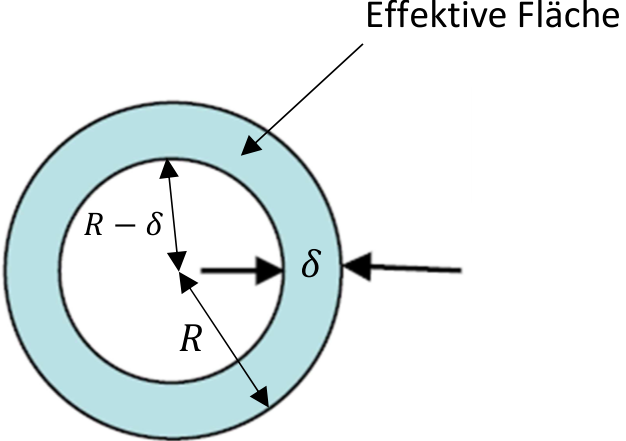
\includegraphics[width=.55\columnwidth]{Figures/Skineffekt.png}\\
%         {\footnotesize$\sigma/\kappa$ : Leitfähigkeit. $[\si{A/Vm}] = [\si{1/\Omega m}]$}
%     \end{minipage}
% }

%\vspace{2cm}

\tikz{
    %Kreise
    \draw[-] (0,0) circle (1);              %äußerer Kreis
    \draw[-] (0,0) circle (0.6);            %innerer Kreis

    %Pfeile
    \draw[latex-latex] (-0.6,0) -- (0,0) node[midway, above]{\tiny{R-$\delta$}};
    \draw[latex-latex] (0,-1) -- (0,0) node at (0,-0.4) [left]{\tiny R};

    \node at (0.8,0)[]{\footnotesize$\delta$};
    \draw[-latex] (0.3,0) -- (0.6,0);
    \draw[latex-] (1,0) -- (1.3,0);

    \draw[latex-] (0.566,0.566) -- (1.2,1.2) node[above, right]{\scriptsize{Effektive Fläche}};

    %Legende
    \node at (-0.8,-1.3)[]{\footnotesize{$\sigma/\kappa$ : Leitfähigkeit [A/Vm] = [1/$\Omega$m]}}




    %--------------------------------------------------------------------
    % %Linien
    % \draw[-] (1,0) -- (1,6);
    % \draw[-] (5,0) -- (5,6);

    % %Pfeile mit Bezeichnungen
    % \draw[->] (3.5,6.5) -- (5,6.5)node[right]{$z$};

    % \draw[->] (1,6) -- (5,5) node[right]{$t_D$} node[midway, above]{$U_{1h}$};
    % %\draw[-] (1,6) -- (3,5.5) node[above]{$U_{1h}$};

    % \draw[->] (5,5) -- (1,4)node[left]{$2t_D$} node[midway, above]{$U_{1r}$};
    % %\draw[-] (5,5) -- (3,4.5) node[above]{$U_{1r}$};

    % \draw[->] (1,4) -- (5,3)node[right]{$3t_D$} node[midway, above]{$U_{2h}$};
    % %\draw[-] (1,4) -- (3,3.5) node[above]{$U_{2h}$};

    % \draw[->] (5,3) -- (1,2)node[left]{$4t_D$} node[midway, above]{$U_{2r}$};
    % %\draw[-] (5,3) -- (3,2.5) node[above]{$U_{2r}$};

    % \draw[->] (1,2) -- (5,1)node[right]{$5t_D$} node[midway, above]{$U_{3h}$};
    % %\draw[-] (1,2) -- (3,1.5) node[above]{$U_{3h}$};


    % \draw[dotted ] (5,1) -- (3,0.5);

    % %Klammern mit Bezeichnungen
    % \draw [black,
    %     decorate,
    %     decoration = {brace,
    %             raise=5pt,
    %             amplitude=5pt}] (1,4.2) --  (1,5.8);
    % \node at(0.5,5)[left]{$U_{1h}$};

    % \draw [black,
    %     decorate,
    %     decoration = {brace,
    %             raise=5pt,
    %             amplitude=5pt}] (5,4.8) --  (5,3.2);
    % \node at (5.5,4)[right]{$U_{1h}(1+r_A)$};

    % \draw [black,
    %     decorate,
    %     decoration = {brace,
    %             raise=5pt,
    %             amplitude=5pt}] (1,2.2) --  (1,3.8);
    % \node at (0.5,3)[left]{$U_{1h}$};
    % \node at (0.5,2.5)[left]{$+(1+r_I)U_{1r}$};

    % \draw [black,
    %     decorate,
    %     decoration = {brace,
    %             raise=5pt,
    %             amplitude=5pt}] (5,2.8) --  (5,1.2);
    % \node at (5.5,2)[right]{$U_{1h}(1+r_A)$};
    % \node at (5.5,1.5)[right]{$+U_{2h}(1+r_A)$};


    % \draw [black,
    %     decorate,
    %     decoration = {brace,
    %             raise=5pt,
    %             amplitude=5pt}] (1,0.2) --  (1,1.8);
    % \node at (0.5,1.5)[left]{$U_{1h}$};
    % \node at (0.5,1)[left]{$+(1+r_I)U_{1r}$};
    % \node at (0.5,0.5)[left]{$+(1+r_I)U_{2r}$};

}

\begin{description}
    \item Äquivalente Leiterschichtdicke (Amp: $A \cdot \frac{1}{e}$):
          \[
              \delta = \frac{1}{\sqrt{\pi\mu\sigma f}} = \sqrt{\frac{2}{\omega\mu\sigma}} \qquad \left[ m \right] \\
          \]

    \item Widerstand/Oberflächenwiderstand:
          \begin{flalign*}
              R_{r\ll\delta}     & = \frac{l}{\sigma \cdot A_{\texttt{eff}}} \\
              R_{r\approx\delta} & =\dfrac{4l}{\sigma \pi d^{2}}             \\
              R_F                & = \dfrac{1}{\sigma \delta}
          \end{flalign*}

    \item \textbf{Feldstärke} verglichen mit der Oberfläche:\\
          \makebox[0pt][l]{
              \begin{minipage}{0.5\columnwidth}
                  \centering
                  \[
                      H\left( x,t\right) = H_{0}\cdot e^{^{-x}/_\delta}\cdot \cos \left( \omega t-\dfrac{x}{\delta}\right)
                  \]
                  \footnotesize analog für $E$-Feld
              \end{minipage}
          }

    \item \textbf{Leistung} verglichen mit der Oberfläche:
          \[
              P\left( x,t\right) = \dfrac{1}{2} \cdot E_{0}\cdot e^{^{-x}/_\delta}\cdot H_{0}\cdot e^{^{-x}/_\delta}
          \]

    \item Amplitude und Phase bezogen auf $\delta$:
          \begin{align*}
              \text{Amplitude: } x   & =\delta \cdot \ln(\text{Dämpfung[ ]}) \\
              \text{Phase: } \varphi & = -\frac{x}{\delta}
          \end{align*}

    \item Effektive Fläche:
          \begin{align*}
              A_{\texttt{eff}} & = A_{\texttt{ges}} - A_{\sigma} = R^2\pi-(R-\sigma)^2\pi \\
                               & = 2\cdot \pi \delta \left( R-\dfrac{\delta }{2}\right)
          \end{align*}
\end{description}

Wenn die Länge nicht gegeben ist oder nach Wieviel \% nimmt der Widerstand bei
einer bestimmten Frequenz, kann dies mit der folgenden Formel berechnet werden:

\begin{description}
    \item Bessel-Funktion:
          \begin{align*}
              \frac{R_{AC}}{R_{DC}} & =
              \begin{dcases}
                  1 + \frac{1}{3}x^4              & \text{für} \qquad x < 1 \\
                  x + \frac{1}{4} + \frac{3}{64x} & \text{für} \qquad x > 1 \\
              \end{dcases} \\
              \frac{X_{AC}}{R_{DC}} & =
              \begin{dcases}
                  x^2\left( 1-\frac{x^4}{6} \right)                               & \text{für} \qquad x < 1 \\
                  x- \frac{3}{64x} + \frac{3}{128x^2} & \text{für} \qquad x > 1 \\
              \end{dcases}
          \end{align*}
          \[
              \boxed{x=\frac{r_0}{2\delta}} \qquad r_0 \hat{=} \textnormal{ Außendurchmesser}
          \]
\end{description}
